\chapter{Introducci'on}\label{cap:intro}
\normalsize
\thispagestyle{plain}

	Los centros de procesamiento de datos (CPD) son uno de los elementos m'as importantes de Internet ya que almacenan, gestionan y procesan la informaci'on que se mueve a trav'es de la red. Durante los 'ultimos a'nos se ha producido un notable incremento en el uso de las Tecnolog'ias de la Informaci'on y Comunicaci'on (TIC), lo que ha originado un aumento del n'umero, rendimiento y capacidad de almacenamiento de los CPDs. En 2014, las empresas EMC e IDC elaboraron un informe \cite{EMC} que sostiene que el tama'no del universo digital en 2013 fue de 4,4 ZB de informaci'on y estima que dicha cifra se incrementará cada a'no, alcanzando en 2020 los 44ZB de informaci'on, un tama'no 10 veces superior al del 2013.
	
	Esta tendencia implica que los CPDs cada vez tendr'an que procesar, almacenar y gestionar m'as informaci'on en el futuro debido al despliegue de nuevo servicios (\textit{cloud computing, IOT, smartcities, e-health...}). Al tener que manejar un mayor volumen de informaci'on, su infraestructura ser'a cada vez m'as grande y tendr'a un mayor n'umero de equipos (servidores, routers, switches, equipos de refrigeraci'on e iluminaci'on...), lo que har'a que su consumo se incremente. En 2014, un informe elaborado por la empresa Yole D'eveloppement \cite{yole} muestra que el consumo de energ'ia mundial de todos los CPDs en ese a'no fue de 352.4 TWh, que equivale al 1.6\% del consumo mundial de energ'ia de ese año, y concluye que si se mantiene esta tendencia, el consumo en 2020 será aproximadamente de 507.9 TWh, lo que supone un incremento del 25\%.

	Todo esto supone un gran impacto econ'omico y medioambiental, por lo que es necesario aplicar medidas que permitan que los centros de datos operen de una forma m'as eficiente y reduzcan su consumo el'ectrico. Para contextualizar correctamente este problema, primero es necesario conocer cómo se distribuye el consumo en un CPD y cómo se mide su eficiencia. Una vez se conoce la distribución del consumo, se van a mencionar las técnicas que se utilizan para reducirlo. Por último, se exponen las soluciones que existen actualmente para tratar este problema y se enfoca el papel de este TFG en dicha solución.

\section{Eficiencia energ'etica en los centros de datos}\label{sec.situacionactual}

	En la figura \ref{fig1_1:cons} se muestran 2 gr'aficos que representan la distribuci'on del consumo de un CPD t'ipico, realizados   por Rychard L. Sawyer \cite{consumo1} y la empresa EYP Mission Critical Facilities \cite{consumo2}, respectivamente. Ambos gr'aficos difieren en el porcentaje y en c'ual es el tipo de infraestructura que m'as consume. Sin embargo, ambos coinciden en que los equipos IT y la refrigeraci'on son los 2 tipos de infraestructura que m'as potencia consumen dentro del CPD, llegando a usar m'as del 75-80\% de la potencia total.

\begin{figure}[htbp]
  \raggedright
	\subfigure{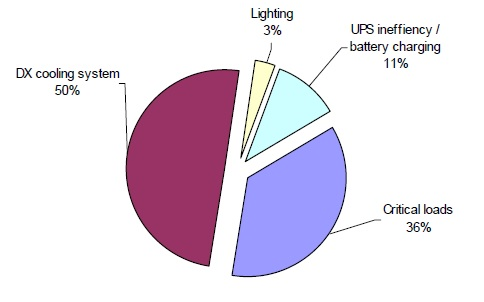
\includegraphics[width=70mm, height=47mm]{imagenes/capitulo1/1_1AConsumo}}
 	\subfigure{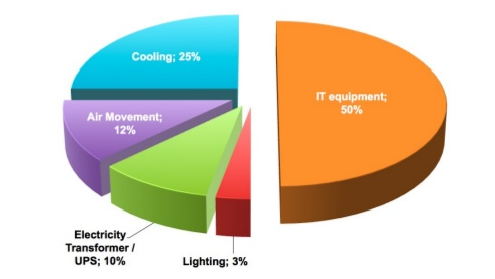
\includegraphics[width=70mm, height=47mm]{imagenes/capitulo1/1_1BConsumo.png}}
   \caption{Distribuci'on del consumo en un centro de datos}
   \label{fig1_1:cons}
\end{figure}

	Para conocer la eficiencia de un CPD, se han desarrollado diferentes m'etricas con el objetivo de medir tanto la eficiencia global del CPD como la eficiencia de cada tipo de consumo. Una de las m'etricas ampliamente usada por la industria para medir la eficiencia global del CPD es el PUE (\textit{Power Usage Effectiveness}) \cite{PUE}. Este par'ametro relaciona la potencia total consumida en el centro de datos con la potencia consumida por los equipos IT. Dicha relaci'on se muestra en la ecuaci'on \ref{ec1.1}.  

\begin{equation}\label{ec1.1}
\normalsize
 PUE= \frac{IT + Cooling + PowerLosses + Building}{IT}
\end{equation}

	Por lo tanto, el objetivo es conseguir reducir este factor lo m'as pr'oximo a la unidad. Para ello, se usan principalmente t'ecnicas de eficiencia energ'etica destinadas a reducir el consumo de los equipos IT o el consumo de refrigeraci'on, ya que son los 2 tipos de consumo que más contribuyen al consumo total y su impacto es más significativo. A continuación se mencionan brevemente algunas de estas técnicas.

\subsection{T'ecnicas de eficiencia en los equipos IT}\label{sec:equiposIT}

	Se consideran equipos IT a los servidores, routers, switches y dem'as elementos que procesan, gestionan y almacenan la informaci'on. Se han desarrollado t'ecnicas tanto a nivel \textbf{hardware} como a nivel \textbf{software} \cite{ITEfficiency} para reducir su consumo. 

	Desde el punto de vista \textbf{hardware}, se usan técnicas como DVFS (\textit{Dynamic Voltage Frecuency Scaling}) \cite{DVFS} y DPM (\textit{Dynamic Power Management}) \cite{DPM}. DVFS es una técnica que pemite reducir el consumo de los procesadores mediante la reducci'on de la tensi'on de alimentaci'on y la frecuencia de la CPU, seg'un la carga de trabajo del procesador. Esta redución se basa en la relacci'on cuadr'atica que existe entre la potencia consumida y la tensi'on de alimentaci'on de los circuitos ($ p\propto C*V^{2}*f$). Por otro lado, DPM se basa en la reducci'on del consumo de potencia ajustando din'amicamente las prestaciones del sistema. Esta t'ecnica puede ser implementada tanto a nivel de circuito como de sistema.

	Desde el punto de vista \textbf{software}, una de las t'ecnicas m'as utilizadas es la virtualizaci'on. La virtualizaci'on permite  que un servidor f'isico albergue m'ultiples m'aquinas virtuales (VMs) independientes y haciendo que sea transparente el movimiento de cargas de trabajo entre un servidor y otro. Para ello, se desarrollan algoritmos \cite{VM} basados en recolocar de forma din'amica las m'aquinas virtuales entre los diferentes nodos f'isicos, teniendo en cuenta criterios de consumo. De este modo, se pretende aumentar el uso de los recursos del sistema y minimizar el n'umero de nodos f'isicos que est'an activos, teniendo en cuenta la carga de trabajo que hay en cada momento y buscando el ahorro energ'etico.

\subsection{T'ecnicas de eficiencia en la refrigeraci'on}\label{sec:refrigeracion}
 
	La refrigeraci'on est'a formada por la unidad de refrigeraci'on, los ventiladores, las canalizaciones y dem'as elementos que permiten que fluya el aire por el CPD. Para reducir el consumo en esta infraestructura, existe un especial inter'es en t'ecnicas como el \textit{free cooling} o abordar el problema del sobreenfriamiento u \textit{overcooling}.

	 El \textit{free cooling} \cite{FreeCooling} consiste en utilizar el aire del exterior para refrigerar la sala, en lugar de usar el sistema de refrigeraci'on. Cuando la temperatura del exterior es inferior a la temperatura del CPD, el aire caliente fluye hacia el exterior de forma natural, por lo que se puede evitar el uso del comprensor y se produce un  importante ahorro de energ'ia.

	El \textit{overcooling} \cite{OverCooling} es un problema que se basa en el sobreenfriamiento de los equipos. La temperatura del aire acondicionado se fija a partir de la potencia térmica máxima que tiene que disipar el sistema de refrigeración cuando el CPD encuentra en el momento de m'aximo funcionamiento. Este enfoque supone un desaprovechamiento de la energ'ia, ya que el CPD no está siempre a pleno funcionamiento. Si se calcula la temperatura a la que debe funcionar el aire acondicionado en funci'on de la carga del CPD, se puede aumentar en ocasiones la temperatura de salida del aire acondicionado y reducir su consumo. Sin embargo, esto puede provocar un aumento en la temperatura de la sala y de los componentes, lo que provoca un aumento de las corrientes de fugas \cite{cfugas}, que no son despreciables, y el aumento del consumo de los equipos.

\section{ Enfoque ciber-f'isico}\label{sec:enfoque}

	Analizando las técnicas anteriormente mencionadas, se observa que dicha técnicas no pueden ser utilizadas de manera aislada, ya que pueden provocar efectos no deseados sobre otros tipos de consumo. Por tanto, es necesario utilizar dichas t'ecnicas de una forma conjunta y coordinada para conseguir que el CPD funcione de manera 'optima, es decir, consumiendo la menor cantidad de energ'ia posible en cada momento.

	El presente TFG forma parte de una l'inea de investigaci'on desarrollada por el equipo de optimizaci'on energ'etica en centros de datos del Laboratorio de Sistemas Integrados \textit{GreenLSI} \cite{GreenLSI}, perteneciente al Departamento de Ingeniería Electrónica (DIE) de la ETSIT-UPM. 

	En ella se expone el problema energ'etico que hay en los CPDs y afirma que hay que tratar ese problema mediante la aplicaci'on conjunta de t'ecnicas de eficiencia energ'etica que permitan reducir el consumo de los equipos y de refrigeraci'on \cite{RespConj}. Adem'as, considera que es necesario la monitorizaci'on del CPD \cite{Monitorizacion} para que dichas t'ecnicas puedan adaptarse de forma din'amica a la carga computacional del CPD y a las condiciones del entorno, pudiendo aplicar en todo momento la configuraci'on m'as eficiente. En la figura \ref{fig1_2:esq} se muestra el esquema del modelo elaborado por \textit{GreenLSI}.

\begin{figure}[htbp]
  \centering
  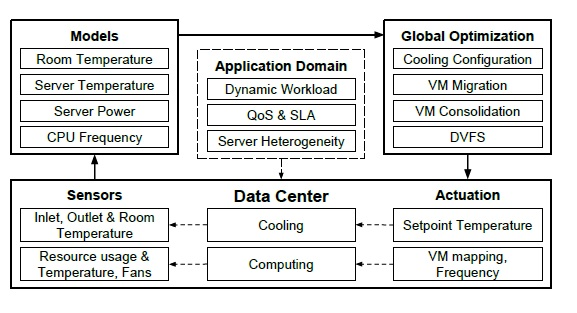
\includegraphics[width=100mm, height=49mm]{imagenes/capitulo1/1_2Esquema}
   \caption{Esquema del sistema de optimizaci'on. Fuente:\cite{Esquema}}
   \label{fig1_2:esq}
\end{figure}
	
	La soluci'on expuesta por \textit{GreenLSI} se basa en un sistema de monitorizaci'on y actuaci'on del CPD. Este sistema consta de una red de sensores distribuidos por el CPD que recoge datos de variables relacionadas con el consumo del CPD, tanto del entorno (temperatura, humedad, presi'on...) como de los equipos (frecuencia de la CPU, temperatura del equipo...). Por otro lado, se han elaborado una serie de modelos \cite{Modelos} que permiten estimar el valor de ciertos par'ametros relacionados con el consumo (temperatura de la sala, temperatura de los servidores, potencia de los servidores...).

	Con la informaci'on proporcionada por los sensores y utilizando los modelos de estimación, se realizan una serie de predicciones sobre el estado del CPD. Después, con las predicciones obtenidas, se realizan distintas optimizaciones tanto a nivel hardware como software, con el objetivo de que el CPD tenga un consumo 'optimo en ese estado. Por 'ultimo, se aplican esas optimizaciones realizando diferentes acciones sobre los elementos que conforman el CPD, ya sean los equipos IT o el sistema de refrigeraci'on. 

	En la figura \ref{fig1_2:esq} puede verse que una de las optimizaciones realizadas es la configuración de la refrigeración o \textit{cooling configuration}. Esta optimización consiste en ajustar la temperatura de la sala en base al estado del CPD y evitar el problema de sobreenfriamento de los equipos, con el objetivo de lograr un ahorro energético en el consumo global. Para ello, se irá modificando la temperatura de funcionamiento del sistema de refrigeración o \textit{setpoint}. Este trabajo se centrará en aplicar dicha optimación.

\section{Objetivos y fases del trabajo}\label{sec:obj}

	El propósito de este trabajo es diseñar un sistema de actuación que permita controlar la temperatura de la sala y fijarla en todo momento al valor proporcionado por el sistema de optimización energética. El sistema irá modificando el \textit{setpoint} del sistema refrigeración para lograr que la sala alcance la temperatura óptima. Para ello, el sistema de actuación debe tener las siguientes características:

	\begin{enumerate}
	\item\textbf{Autonomía:} el actuador tiene que llevar a cabo las acciones necesarias para fijar la temperatura de la sala sin intervención humana.
	\item\textbf{Dinámico:} el actuador debe responder a los cambios que se produzcan en la temperatura de optimización. Dicha respuesta debe hacerse a la mayor brevedad posible y teniendo en cuenta las limitaciones físicas que pudiera haber.
	\item\textbf{Estabilidad:} el actuador debe funcionar de una forma correcta, segura y sin comportamientos que puedan afectar al correcto funcionamiento del CPD.
	\item\textbf{No invasivo:} el funcionamiento del actuador no debe influir en el comportamiento normal de cada uno de los elementos del CPD.
	\item\textbf{Adaptable:} el actuador debe poder configurarse para que pueda ser usado en diferentes centros de datos. Dicha configuración tiene que ser sencilla y que implique el menor número de cambios posibles.
	\end{enumerate}

	En cuanto a las fases del trabajo, primero se exponen en el capítulo \ref{cap:estadoarte} los principales sistemas de control usados en la industria para controlar la temperatura. Después, en el capítulo \ref{cap:bancopruebas} se caracteriza el banco de pruebas usado para probar el actuador. A continuación, en los capítulos \ref{cap:dise'no} y \ref{cap:implementacion} se detallan todas las cuestiones relacionadas con el diseño y la implementación del actuador, respectivamente. Luego, en el capítulo \ref{cap:test} se muestran los experimentos realizados y se analizan los resultados obtenidos. Por último, en el capítulo \ref{cap:conclusiones}, se exponen las principales conclusiones de este trabajo y cuáles son sus principales líneas futuras.
